\documentclass[a4paper,12pt]{report}
\usepackage{CJKutf8, color, times, titlesec, geometry, indentfirst, 
            tcolorbox, smartdiagram, amssymb, graphicx, svg, pdfpages, minted, listings}
\usepackage[backend=biber,style=numeric,sorting=none]{biblatex}
\addbibresource{report.bib}
\usepackage[colorlinks=true, linkcolor=blue]{hyperref}
\usepackage[utf8]{inputenc}
\usepackage[T1]{fontenc}
\usepackage{bookmark}
\geometry{margin=2cm}
\setlength{\parindent}{2em}

\newcommand{\TODO}[1]{\textbf{<TODO: #1 will be inserted here.>}}

\definecolor{mygreen}{rgb}{0,0.6,0}
\definecolor{mygray}{rgb}{0.5,0.5,0.5}
\definecolor{mymauve}{rgb}{0.58,0,0.82}

% listing code conf.
\lstset{ 
  backgroundcolor=\color{white},   % choose the background color; you must add \usepackage{color} or \usepackage{xcolor}; should come as last argument
  basicstyle=\ttfamily\footnotesize,% the size of the fonts that are used for the code
  breakatwhitespace=false,         % sets if automatic breaks should only happen at whitespace
  breaklines=true,                 % sets automatic line breaking
  captionpos=b,                    % sets the caption-position to bottom
  commentstyle=\color{mygreen},    % comment style
  deletekeywords={...},            % if you want to delete keywords from the given language
  escapeinside={\%*}{*)},          % if you want to add LaTeX within your code
  extendedchars=true,              % lets you use non-ASCII characters; for 8-bits encodings only, does not work with UTF-8
  frame=single,	                   % adds a frame around the code
  keepspaces=true,                 % keeps spaces in text, useful for keeping indentation of code (possibly needs columns=flexible)
  keywordstyle=\color{red},        % keyword style
  morekeywords={*,...},            % if you want to add more keywords to the set
  numbers=left,                    % where to put the line-numbers; possible values are (none, left, right)
  numbersep=5pt,                   % how far the line-numbers are from the code
  numberstyle=\tiny\color{mygray}, % the style that is used for the line-numbers
  rulecolor=\color{black},         % if not set, the frame-color may be changed on line-breaks within not-black text (e.g. comments (green here))
  showspaces=false,                % show spaces everywhere adding particular underscores; it overrides 'showstringspaces'
  showstringspaces=false,          % underline spaces within strings only
  showtabs=false,                  % show tabs within strings adding particular underscores
  stepnumber=1,                    % the step between two line-numbers. If it's 1, each line will be numbered
  stringstyle=\color{mymauve},     % string literal style
  tabsize=4,	                     % sets default tabsize to ˋ spaces
  title=\lstname,                  % show the filename of files included with \lstinputlisting; also try caption instead of title
  extendedchars=true,
}

\input{lib/codeblock}

\title{{
\LARGE 健康資訊交換系統中之容器安全\\
\Large The Container Security in Healthcare Data Exchange System
\newline
\newline
\newline
\newline
\large
國立中山大學資訊工程學系\\
Department of Computer Science and Engineering\\
National Sun-Yet-San University, Taiwan \\
110 學年度大學部專題製作競賽 \\
Bachelor's degree graduation project in 2021\\
}}

\author{
Author: Chih-Hsuan Yang (B073040047)\\
Advisor: Chun-I Fan
}

\linespread{1.5}
\begin{document}
\begin{CJK*}{UTF8}{bkai}
  \maketitle
  \includepdf{contribute.pdf}
  \chapter*{Abstract}
\addcontentsline{toc}{chapter}{Abstract}

This is a string.


  {
    \linespread{1}\selectfont
    \tableofcontents
  }
  \chapter{Introduction}

\section{Container and Linux Kernel}

The container is a secondary product of the operating system in the past 20 years.
The FreeBSD develops `Jails' in 1999, and the Solaris develops `Zones' in 2004.
Linux also took this idea into the Linux kernel, which is named cgroups (2007),
the capabilities (2003), and seccomp (2005). However, why the Linux breaks this
technology into many parts? This is because they had discussed:
"Why Should a System Administrator Upgrade?" in 2001
\footnote{Version 2.4 of the LINUX KERNEL--Why Should a System Administrator Upgrade?
    \url{https://www.informit.com/articles/article.aspx?p=20667}}.
The Linux kernel almost entered the development path of "upgrade for demand" like
Microsoft Windows, and deviated from the original path of "providing a mechanism
but not a strategy" of the original Linux kernel.

While Linux were spreading in various server or distributed system, the
Linux community got more pull requests to solved the scalability and virtualization
issues \cite{267148}. However, they avoided confusion caused by multiple meanings of
the term "container" in the Linux kernel context. In kernel version 2.6.24 (2007)
\footnote{Notes from a container: \url{https://lwn.net/Articles/256389/}},
control groups functionality was merged into the mainline,
which is designed for an administrator (or administrative daemon) to organize processes
into hierarchies of containers; each hierarchy is managed by a subsystem. Moreover, the
cgroups was rewrote into cgroups-v2 in Linux kernel 4.5 (2015)
\footnote{Control Group v2: \url{https://www.kernel.org/doc/Documentation/cgroup-v2.txt}}.

The first and most complete implementation of the Linux container manager was LXC
(Linux Containers). It was implemented in 2008 using cgroups and namespaces,
and it runs on a single Linux kernel without requiring any patches. LXC provides
a new view and imagination of virtualized services without any hypervisor. In 2016,
Docker replaced LXC with "libcontainer", which was written in the Go programming language.
Docker combined features in a new, more attractive way and made Linux containers popular.

The secondary product of the operating system, containers, offering many advantages:
they enable you to "build once, run anywhere." Docker does this by bundling
applications with all their dependencies into one package and isolating applications
from the rest of the machine on which they're running. Therefore, this research
is based on docker container to propose a scheme of healthcare data exchange system's
security.

\section{FHIR}
FHIR is a standard for healthcare data exchange. The FHIR standard will be used in
Taiwan in the near future. FHIR will be used to provide PHR (Personal Healthcare Records)
in Taiwan. Therefore, we choose the most popular standard "FHIR" for the target of
the healthcare data exchange system.

\subsection{RESTful API and Data Structure}
REST (Representational State Transfer) is a stateless reliable web API, which is based
on HTTP methods to access resources or data via URL parameters and the use of JSON or
XML format to transmit queries. Because the RESTful is stateless, the client should
keep their information (i.e. cookies) by themself.

FHIR has features: RESTful and data structure, make our research and benchmarks more accurate
and reliable.
Statelessness is a developer-friendly feature, the developer and the tester would not
to design a complex state machine on the server-side or generating test files. And the FHIR
takes RESTful as standard. Moreover, FHIR standard declared the `StructureDefinition'
\footnote{FHIR Resource Structure Definition: \url{http://www.hl7.org/fhir/structuredefinition.html}}.
These structure definitions are used to describe both the content defined in the FHIR
specification itself - Resources, data types, the underlying infrastructural types, and
also are used to describe how these structures are used in implementations.

\subsection{Why IBM FHIR server}
There are many applications using IBM's FHIR server as the base component of the EHR
(Electronic Health Records) system to communicate with the other various databases.
Take it for example that the NextCloud's EHR service, Taipei Veterans General Hospital,
and AWS Cloud are using the FHIR server in a container for subroutine service.
NextCloud is an open-source and self-hosted productivity platform for users.
Many people caring about their privacy issues distrust the FAAMG (Facebook,
Amazon, Apple, Microsoft, Google), so they are using NextCloud to keep their privacy
on their own. Therefore, they are eager to have a secure EHR system for their
PHR
\footnote{\href{https://www.youtube.com/watch?v=AAP4N3KyLmM}{Richard Stallman talks about IoT}}.

The benefits of providing IBM FHIR container security in our study are providing
secure protection testing, methods, and performance evaluation for FHIR services provided by
well-known international company (IBM). This research will provide an important reference for
commercial projects for the health information exchange system practiced by medical
institutions in Taiwan.

% \section{Data and Privacy}
% Medical privacy is keeping patient records secure and confidential. In the field of software 
% engineering, each person's biological information is just a piece of data. But for living people, 
% bioinformatics is a basic human right to their human dignity.
  \chapter{Related Works}

\section{Collecting System Calls}

\section{Find-granted Permission Control}

\section{Recently Exploited Vulnerabilities}
\subsection{Five Stage of Malware}

\section{Virtual Environment Performance Benchmark}
  \chapter{Preliminary}

\section{Container's Components}
\subsection{Namespaces}
\subsection{Cgroups}
\subsection{Seccomp}

\section{Programs in Execution}
\subsection{The task\_struct in Kernel}
\subsection{Capabilities}

\section{User Mode Linux}
\subsection{Sandbox Security}
\subsection{gVisor}

\section{The (e)BPF}

  \chapter{Proposed Scheme}

\section{Workflow}
We proposed a CI/CD workflow to guarantee runtime enforcement of policies 
in figure \ref{fig:workflow}.

\begin{figure}
    \centering
    \smartdiagramset{
        module minimum width=3cm,
        text width=2.5cm,
    }
    \smartdiagram[circular diagram:clockwise]{
        Scan base, Sign, Image checking, Start policy, Runtime enforcement
    }
    \label{fig:workflow}
    \caption{Contiguous Integration and Contiguous Deployment}
\end{figure}

\subsection{Scan Base Image}
\subsection{Building and Signing}
\subsection{Check Image and Policy}
\subsection{Enforce the Policy}

\section{Rolling Updates}
  \chapter{Analysis and Benchmark}

\section{Analysis}
\subsection{Attacking Surface}
\subsection{Time Consuming}
\subsection{Statistics}
Figure \ref{hist} is the FHIR server's all system calls in 
BoSC\cite{1495942} and the number of called times.
\begin{figure}
    \centering
    \includegraphics[width=\textwidth]{src/hist.png}
    \label{hist}
    \caption{All the system calls which the FHIR called times}
\end{figure}



\section{Benchmark}
\subsection{Latency}
Figure \ref{conc} is the concurrent processes transporting time
difference in container and virtual machine.
\begin{figure}
    \centering
    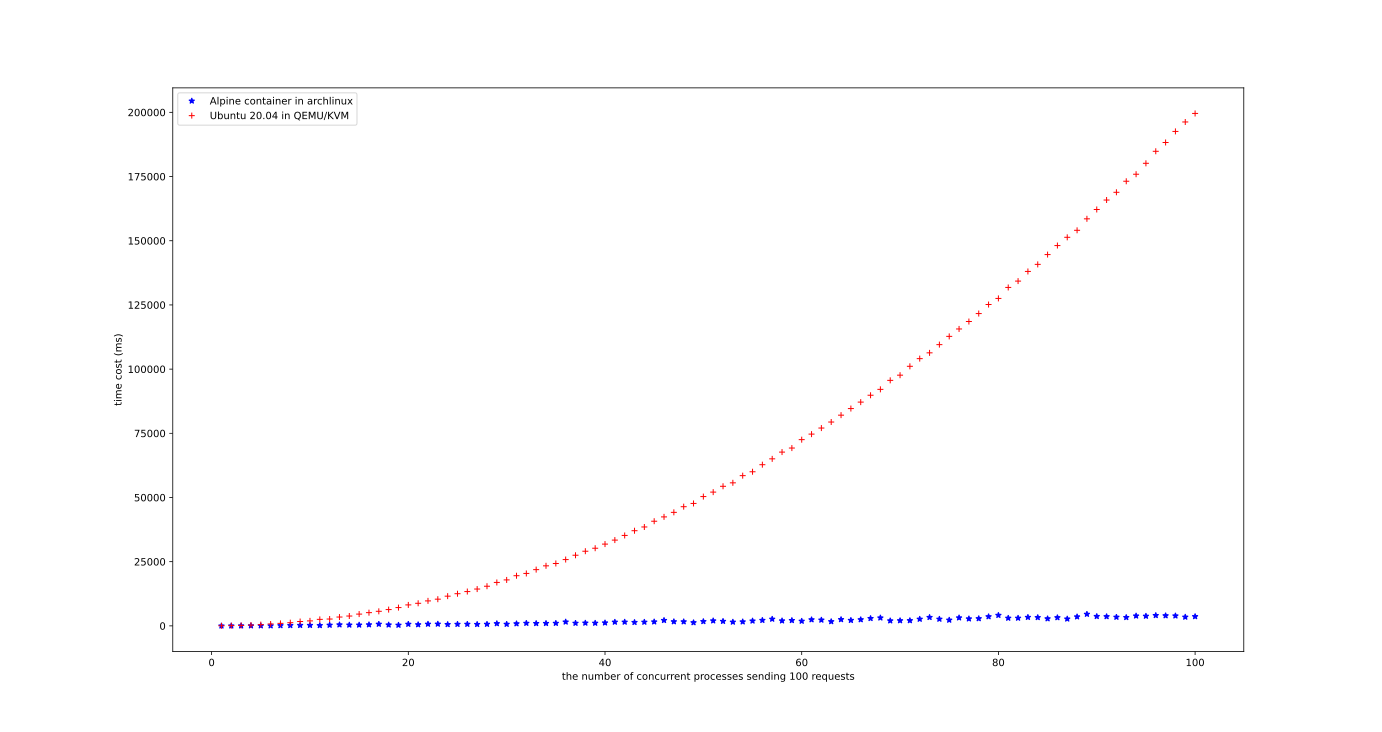
\includegraphics[width=\textwidth]{src/concurrent.png}
    \label{conc}
    \caption{Concurrent processes transporting time}
\end{figure}

\subsection{Throughput}
TBD\dots
  \section{Conclusion}

We can see that the comparison results in virtual machine and container are
significantly indifferent order of time-consuming. There is no existence
of the gVisor's result because the gVisor was not able to launch the
IBM/FHIR server system, which is the target of our research.
We also expect that the gVisor might run faster significantly than the virtual
machine; however, our target cannot be launched successfully in
gVisor's sandbox.
We thought that there might have been some race condition bugs via JWE (JAVA Web
Engine) in gVisor, such that the gVisor did not do well in supporting all system calls.

And the time complexity of the virtual machine is significantly different from
the container. We propose a hypothesis of the time complexity of the virtual
machine, because there are more page fault events and the throughput limitation
of virtual machine device driver \cite{10.5555/1267569.1267570,7095802}.

The proposed scheme is nearly zero-overhead protection in the kernel, and
the policy is auto-generated and conformed in the build time. It could help
developers to deploy into a secure environment with no pain. This paper also
benchmarked the protection via virtual machine and our proposed scheme in
the container. It can be concluded that it is a good solution if we want
low latency and security.



  \nocite{*}
  \linespread{1}\selectfont
  \printbibliography[title=Reference]
  \addcontentsline{toc}{chapter}{Reference}

\end{CJK*}
\end{document}
